\documentclass[ignorenonframetext,]{beamer}
\setbeamertemplate{caption}[numbered]
\setbeamertemplate{caption label separator}{: }
\setbeamercolor{caption name}{fg=normal text.fg}
\beamertemplatenavigationsymbolsempty
\usepackage{lmodern}
\usepackage{amssymb,amsmath}
\usepackage{ifxetex,ifluatex}
\usepackage{fixltx2e} % provides \textsubscript
\ifnum 0\ifxetex 1\fi\ifluatex 1\fi=0 % if pdftex
  \usepackage[T1]{fontenc}
  \usepackage[utf8]{inputenc}
\else % if luatex or xelatex
  \ifxetex
    \usepackage{mathspec}
  \else
    \usepackage{fontspec}
  \fi
  \defaultfontfeatures{Ligatures=TeX,Scale=MatchLowercase}
\fi
\usetheme[]{Warsaw}
\usecolortheme{dolphin}
\usefonttheme{structuresmallcapsserif}
% use upquote if available, for straight quotes in verbatim environments
\IfFileExists{upquote.sty}{\usepackage{upquote}}{}
% use microtype if available
\IfFileExists{microtype.sty}{%
\usepackage{microtype}
\UseMicrotypeSet[protrusion]{basicmath} % disable protrusion for tt fonts
}{}
\newif\ifbibliography
\hypersetup{
            pdftitle={Intro Datenanalyse mit R - Dein Freund das GUI},
            pdfauthor={Jan-Philipp Kolb},
            pdfborder={0 0 0},
            breaklinks=true}
\urlstyle{same}  % don't use monospace font for urls
\usepackage{graphicx,grffile}
\makeatletter
\def\maxwidth{\ifdim\Gin@nat@width>\linewidth\linewidth\else\Gin@nat@width\fi}
\def\maxheight{\ifdim\Gin@nat@height>\textheight0.8\textheight\else\Gin@nat@height\fi}
\makeatother
% Scale images if necessary, so that they will not overflow the page
% margins by default, and it is still possible to overwrite the defaults
% using explicit options in \includegraphics[width, height, ...]{}
\setkeys{Gin}{width=\maxwidth,height=\maxheight,keepaspectratio}

% Prevent slide breaks in the middle of a paragraph:
\widowpenalties 1 10000
\raggedbottom

\AtBeginPart{
  \let\insertpartnumber\relax
  \let\partname\relax
  \frame{\partpage}
}
\AtBeginSection{
  \ifbibliography
  \else
    \let\insertsectionnumber\relax
    \let\sectionname\relax
    \frame{\sectionpage}
  \fi
}
\AtBeginSubsection{
  \let\insertsubsectionnumber\relax
  \let\subsectionname\relax
  \frame{\subsectionpage}
}

\setlength{\parindent}{0pt}
\setlength{\parskip}{6pt plus 2pt minus 1pt}
\setlength{\emergencystretch}{3em}  % prevent overfull lines
\providecommand{\tightlist}{%
  \setlength{\itemsep}{0pt}\setlength{\parskip}{0pt}}
\setcounter{secnumdepth}{0}

\title{Intro Datenanalyse mit R - Dein Freund das GUI}
\author{Jan-Philipp Kolb}
\date{05 Juni, 2019}

\begin{document}
\frame{\titlepage}

\begin{frame}{Open Source Programm R}

\begin{itemize}
\item
  R ist eine freie, nicht-kommerzielle Implementierung der
  Programmiersprache S (von AT\&T Bell Laboratories entwickelt)
\item
  Freie Beteiligung - modularer Aufbau (immer mehr Erweiterungspakete)
\item
  Der Download ist auf dieser Seite möglich:
\end{itemize}

\url{https://cran.r-project.org/}

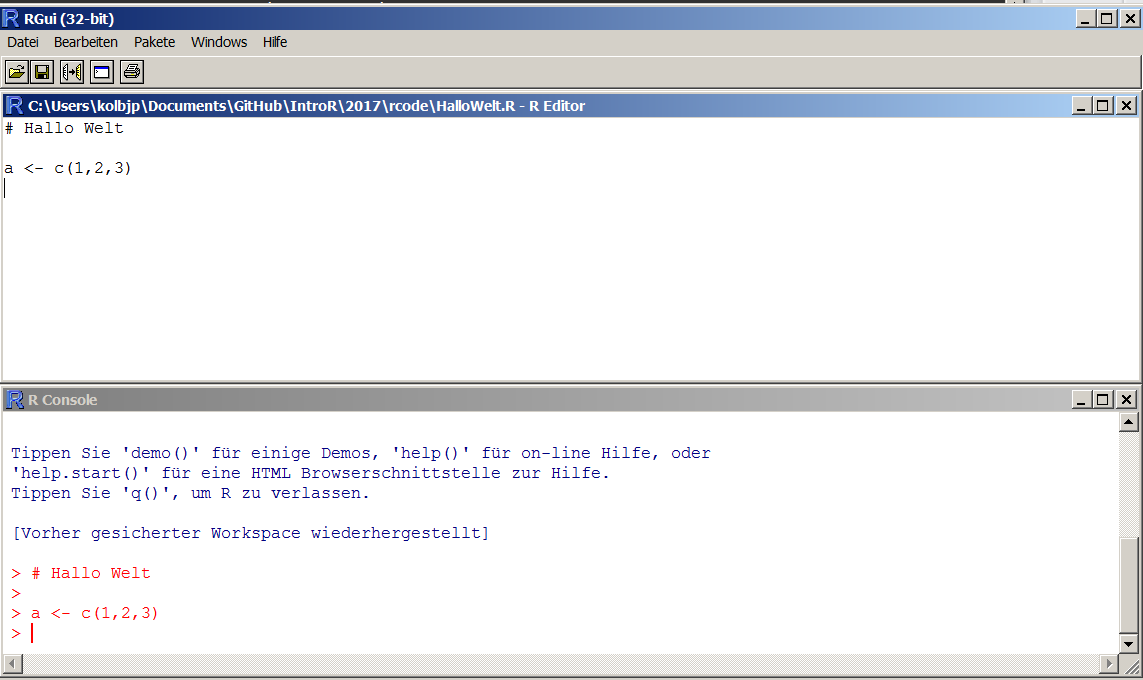
\includegraphics{figure/BasisR.PNG}

\end{frame}

\begin{frame}{Graphisches User Interface}

Aber die meisten Menschen nutzen einen Editor oder ein graphical user
interface (GUI).

Aus den folgenden Gründen:

\begin{itemize}
\tightlist
\item
  Syntax highlighting
\item
  Auto-Vervollständigung
\item
  Bessere Übersicht über Graphiken, Bibliotheken
\end{itemize}

\end{frame}

\begin{frame}{Verschiedene GUIs}

\begin{itemize}
\item
  \href{https://projects.gnome.org/gedit/}{Gedit} mit R-spezifischen
  Add-ons für Linux
\item
  \href{http://www.gnu.org/software/emacs/}{Emacs}
\item
  \href{http://www.sciviews.org/Tinn-R/}{TinnR}
\item
  Ich nutze \href{https://www.rstudio.com/}{Rstudio!}
\end{itemize}

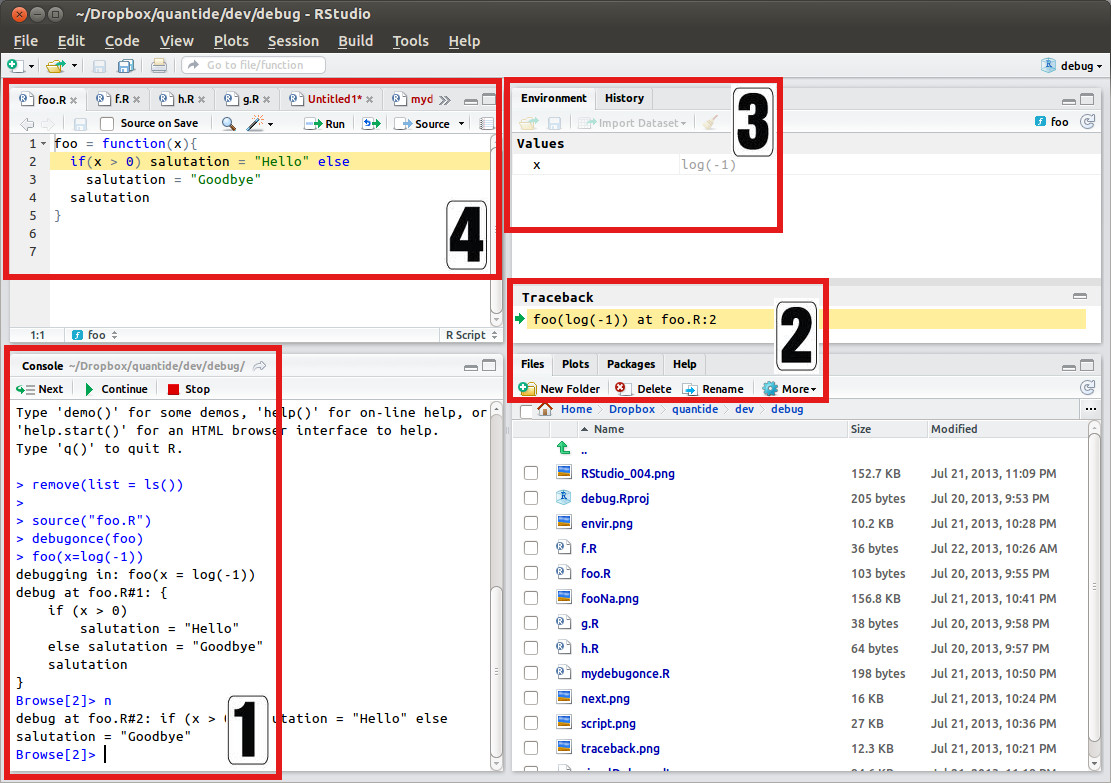
\includegraphics{figure/0_overall.jpg}

\end{frame}

\begin{frame}{Links zu Rstudio}

\begin{itemize}
\item
  Sechs
  \href{http://www.r-bloggers.com/top-6-reasons-you-need-to-be-using-rstudio/}{\textbf{Gründe}}
  Rstudio zu nutzen.
\item
  Wie man Rstudio
  \href{https://support.rstudio.com/hc/en-us/sections/200107586-Using-RStudio}{\textbf{nutzen
  kann.}} - kleine Artikel zu verschiedenen Themen - bspw. Debugging,
  Paketmanagement oder Shortcuts.
\item
  \href{https://support.rstudio.com/hc/en-us/articles/200549016-Customizing-RStudio}{\textbf{RStudio
  einrichten}} - Im Menü gibt es unter Tools \textgreater{} Optionen
  eine Reihe von Einstellungen - wozu diese gut sind, wird in diesem
  Artikel erklärt.
\item
  \href{https://dss.princeton.edu/training/RStudio101.pdf}{\textbf{Einführung
  in RStudio}} - hier werden die ersten Schritte in RStudio ausführlich
  erklärt. 
\item
  \href{https://github.com/rstudio/cheatsheets/raw/master/rstudio-ide.pdf}{\textbf{RStudio
  Cheatsheet}} - Übersichtliche Darstellung von Funktionen in RStudio
\end{itemize}

\end{frame}

\end{document}
